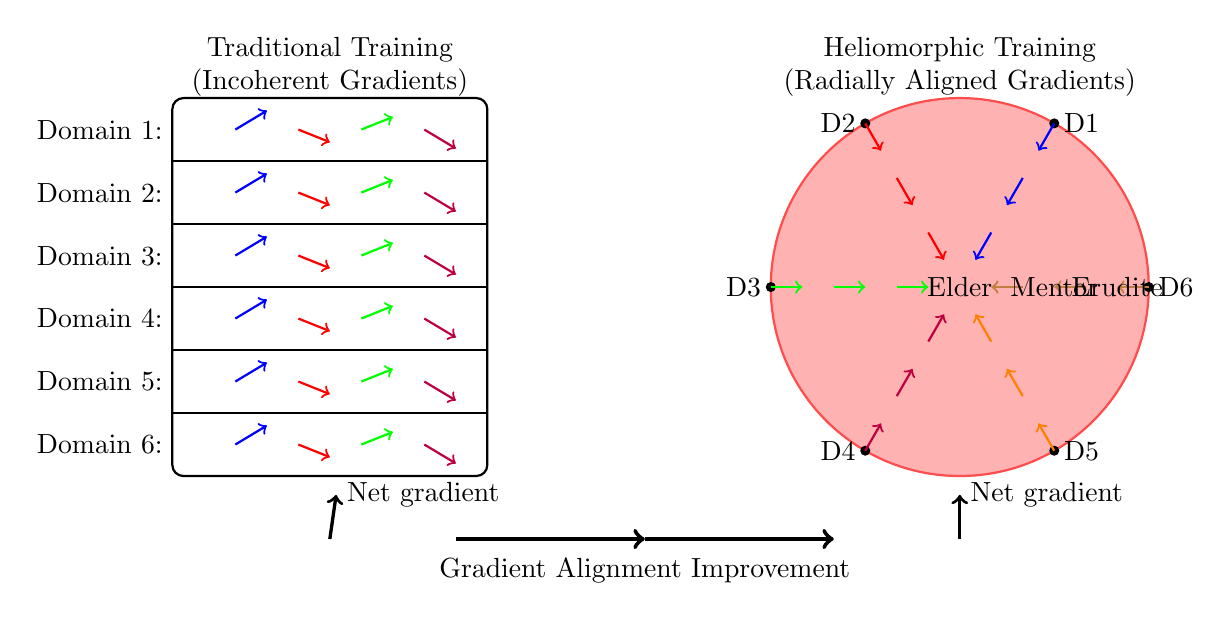
\begin{tikzpicture}[scale=0.8]
  % Define colors
  \colorlet{eldershell}{blue!30}
  \colorlet{mentorshell}{green!40}
  \colorlet{eruditeshell}{red!30}
  \colorlet{elderborder}{blue!70}
  \colorlet{mentorborder}{green!70}
  \colorlet{eruditeborder}{red!70}
  
  % Create two diagrams side by side
  % Holomorphic approach - Traditional training
  \begin{scope}[shift={(-5,0)}]
    % Draw architecture
    \draw[thick, rounded corners] (-2.5,-3) rectangle (2.5,3);
    
    % Layers
    \draw[thick] (-2.5,-2) -- (2.5,-2);
    \draw[thick] (-2.5,-1) -- (2.5,-1);
    \draw[thick] (-2.5,0) -- (2.5,0);
    \draw[thick] (-2.5,1) -- (2.5,1);
    \draw[thick] (-2.5,2) -- (2.5,2);
    
    % Domain labels
    \node[left] at (-2.5,2.5) {Domain 1:};
    \node[left] at (-2.5,1.5) {Domain 2:};
    \node[left] at (-2.5,0.5) {Domain 3:};
    \node[left] at (-2.5,-0.5) {Domain 4:};
    \node[left] at (-2.5,-1.5) {Domain 5:};
    \node[left] at (-2.5,-2.5) {Domain 6:};
    
    % Gradients (random directions)
    \draw[->, thick, blue] (-1.5,2.5) -- (-1,2.8);
    \draw[->, thick, red] (-0.5,2.5) -- (0,2.3);
    \draw[->, thick, green] (0.5,2.5) -- (1,2.7);
    \draw[->, thick, purple] (1.5,2.5) -- (2,2.2);
    
    \draw[->, thick, blue] (-1.5,1.5) -- (-1,1.8);
    \draw[->, thick, red] (-0.5,1.5) -- (0,1.3);
    \draw[->, thick, green] (0.5,1.5) -- (1,1.7);
    \draw[->, thick, purple] (1.5,1.5) -- (2,1.2);
    
    \draw[->, thick, blue] (-1.5,0.5) -- (-1,0.8);
    \draw[->, thick, red] (-0.5,0.5) -- (0,0.3);
    \draw[->, thick, green] (0.5,0.5) -- (1,0.7);
    \draw[->, thick, purple] (1.5,0.5) -- (2,0.2);
    
    \draw[->, thick, blue] (-1.5,-0.5) -- (-1,-0.2);
    \draw[->, thick, red] (-0.5,-0.5) -- (0,-0.7);
    \draw[->, thick, green] (0.5,-0.5) -- (1,-0.3);
    \draw[->, thick, purple] (1.5,-0.5) -- (2,-0.8);
    
    \draw[->, thick, blue] (-1.5,-1.5) -- (-1,-1.2);
    \draw[->, thick, red] (-0.5,-1.5) -- (0,-1.7);
    \draw[->, thick, green] (0.5,-1.5) -- (1,-1.3);
    \draw[->, thick, purple] (1.5,-1.5) -- (2,-1.8);
    
    \draw[->, thick, blue] (-1.5,-2.5) -- (-1,-2.2);
    \draw[->, thick, red] (-0.5,-2.5) -- (0,-2.7);
    \draw[->, thick, green] (0.5,-2.5) -- (1,-2.3);
    \draw[->, thick, purple] (1.5,-2.5) -- (2,-2.8);
    
    % Title
    \node[align=center] at (0,3.5) {Traditional Training\\(Incoherent Gradients)};
    
    % Net gradient
    \draw[->, very thick, black] (0,-4) -- (0.1,-3.3) node[right] {Net gradient};
  \end{scope}
  
  % Heliomorphic approach
  \begin{scope}[shift={(5,0)}]
    % Draw concentric shells
    \draw[elderborder, thick, fill=eldershell] (0,0) circle (1);
    \draw[mentorborder, thick, fill=mentorshell] (0,0) circle (2);
    \draw[eruditeborder, thick, fill=eruditeshell] (0,0) circle (3);
    
    % Domain points
    \filldraw (60:3) circle (2pt) node[right] {D1};
    \filldraw (120:3) circle (2pt) node[left] {D2};
    \filldraw (180:3) circle (2pt) node[left] {D3};
    \filldraw (240:3) circle (2pt) node[left] {D4};
    \filldraw (300:3) circle (2pt) node[right] {D5};
    \filldraw (360:3) circle (2pt) node[right] {D6};
    
    % Gradients (now aligned radially)
    \draw[->, thick, blue] (60:3) -- (60:2.5);
    \draw[->, thick, red] (120:3) -- (120:2.5);
    \draw[->, thick, green] (180:3) -- (180:2.5);
    \draw[->, thick, purple] (240:3) -- (240:2.5);
    \draw[->, thick, orange] (300:3) -- (300:2.5);
    \draw[->, thick, brown] (360:3) -- (360:2.5);
    
    % Second level gradients
    \draw[->, thick, blue] (60:2) -- (60:1.5);
    \draw[->, thick, red] (120:2) -- (120:1.5);
    \draw[->, thick, green] (180:2) -- (180:1.5);
    \draw[->, thick, purple] (240:2) -- (240:1.5);
    \draw[->, thick, orange] (300:2) -- (300:1.5);
    \draw[->, thick, brown] (360:2) -- (360:1.5);
    
    % Core gradients
    \draw[->, thick, blue] (60:1) -- (60:0.5);
    \draw[->, thick, red] (120:1) -- (120:0.5);
    \draw[->, thick, green] (180:1) -- (180:0.5);
    \draw[->, thick, purple] (240:1) -- (240:0.5);
    \draw[->, thick, orange] (300:1) -- (300:0.5);
    \draw[->, thick, brown] (360:1) -- (360:0.5);
    
    % Layer labels
    \node at (0,0) {Elder};
    \node at (0:1.5) {Mentor};
    \node at (0:2.5) {Erudite};
    
    % Title
    \node[align=center] at (0,3.5) {Heliomorphic Training\\(Radially Aligned Gradients)};
    
    % Net gradient
    \draw[->, very thick, black] (0,-4) -- (0,-3.3) node[right] {Net gradient};
  \end{scope}
  
  % Connecting arrow and label
  \draw[<-, ultra thick] (0,-4) -- (-3,-4);
  \draw[->, ultra thick] (0,-4) -- (3,-4);
  \node[align=center] at (0,-4.5) {Gradient Alignment Improvement};
\end{tikzpicture}